\section{Power and the choice of test}\label{sec:power}

Size is only half of the choice. Consider local alternatives $\mu-\mu_0=c\,\sigma n^{H-1}$, under which
$\sqrt n(\bar x-\mu_0)/(\sigma n^{H-1/2})\to Z+c$ while every self-normaliser keeps its null limit. In this section $c$ denotes this drift; critical values are written $q$.

\begin{proposition}[Local power of a finite-dimensional statistic]\label[proposition]{prop:power}
Let the self-normaliser be a finite quadratic form $D_P=\sum_{k=1}^Kw_kV_k^2$ in Gaussian components, let
$V=(Z,V_1,\dots,V_K)\sim N(0,\Sigma)$ with $\Sigma$ positive definite, and let
$A=\operatorname{diag}(1,-q\,w_1,\dots,-q\,w_K)$, where $q$ is the critical value of the squared statistic. Let
$\Sigma=LL^\top$, $L^\top AL=P\Theta P^\top$ and $\psi=\Theta^{-1}P^\top L^\top Ae_1c$. Then the limit power at $c$ is the
noncentral weighted chi-square probability
\[P\Big(\sum_i\Theta_{ii}(\xi_i+\psi_i)^2>0\Big),\qquad \xi_i\ \text{independent standard normal}.\]
\end{proposition}

We evaluate it by the noncentral form of Imhof's inversion \citep{Imh61}. For the fixed-smoothing statistics $K$ is
finite and the power is exact up to quadrature error. The self-normaliser of $T_H$ has infinitely many components; we
truncate it at $J=512$ cosine coordinates (\cref{prop:coords}) and replace the remainder by its mean, so its power is
computed rather than certified. Over every $H$ and $c$ of our grid it changes by at most \pthree{pw-jl-256-512} from
$J=256$ to $J=512$ and by at most \pthree{pw-jl-512-1024} from $J=512$ to $J=1024$. At $c=0$ the computed power equals
the nominal level to within \pthree{pw-c0-maxdev}, and at $H=\frac12$ the fixed-smoothing power equals the noncentral
Student-$t$ power to within \pthree{pw-nct-maxdev} in all \pthree{pw-nct-ncells} cells.

\begin{figure}[tbp]\centering
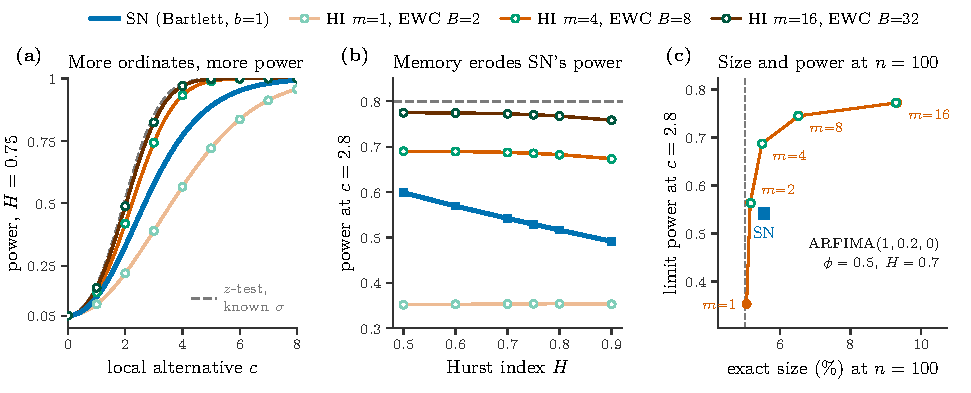
\includegraphics[width=\textwidth]{fig3_power.pdf}
\caption{Limit power and the size--power trade-off. (a)~Power at $H=0.75$ against the local alternative $c$; dashed:
infeasible $z$-test. (b)~Power at $c=2.8$ against $H$. (c)~Power at $c=2.8$ against exact size at $n=100$ under
ARFIMA$(1,0.2,0)$, $\phi=0.5$; open circles: EWC, $B=2m$; square: Bartlett/self-normalised test.}\label{fig:power}
\end{figure}

\Cref{fig:power} shows three regularities.
\emph{(i) Power grows with the number of components.} At $H=0.75$ and $c=2.8$ the power is \pthree{pw-HI1-0.75} for
$m=1$, \pthree{pw-HI4-0.75} for $m=4$ and \pthree{pw-HI16-0.75} for $m=16$, against \pthree{pw-z} for the infeasible
$z$-test that knows the scale $\sigma$ of the partial sums. The fixed-$m$ test with $m$ frequencies and the EWC test with $B=2m$ cosines have the same power to within
\pthree{pw-hi-ewc-maxdiff} at every $H$ and $c$ in our grid.
\emph{(ii) Memory erodes the power of the Bartlett/self-normalised test, but hardly that of the fixed-smoothing tests.}
From $H=\frac12$ to $H=0.9$ the power at $c=2.8$ of the former falls from \pthree{pw-SN-0.50} to \pthree{pw-SN-0.90}; that
of the fixed-$m$ test with $m=16$ changes from \pthree{pw-HI16-0.50} to \pthree{pw-HI16-0.90}.
\emph{(iii) Under short-run dynamics, power costs finite-sample size.} Each additional component raises power and,
in the design of \cref{fig:power}c, the finite-sample distortion; this is the size--power trade-off of \citet{LLS21} in the
long-memory setting.

\paragraph{Which test} With the critical value of the true $H$, the Bartlett/self-normalised test is dominated, in the
sense of a larger exact finite-sample size distortion together with a lower limit power against local alternatives
(power at finite $n$ is not computed here): at
$n=100$, $H=0.7$ and $\phi=0.5$ the fixed-$m$ test with $m=4$ has size \pthree{fn-arfima1p-HI4-0.70-100}\,\% and power
\pthree{pw-HI4-0.70}, against \pthree{fn-arfima1p-SN-0.70-100}\,\% and \pthree{pw-SN-0.70} for the former, and the
fixed-$m$ test with $m=4$ has both the smaller finite-sample size distortion and the higher limit power in
\pthree{dominance-share} of the
\pthree{dominance-ncells} $(H,n,\text{model})$ cells of our design. In limit power alone, the fixed-$m$ test with $m=4$ (EWC, $B=8$) exceeds the
Bartlett/self-normalised test in all \pthree{pw-vsSN-ncells} $(H,c)$ cells of the grid with $c>0$, with $m=2$ ($B=4$)
in \pthree{pw-vsSN-HI2-npos} (\pthree{pw-vsSN-EWC4-npos}), and with $m=1$ ($B=2$) in none. Fixed-smoothing tests with $m\le4$ frequencies, or
EWC tests with $B\in\{4,8\}$, are within \pthree{fn-maxdev-small-100}\,pp of $5\,\%$ for $n\ge100$ in every design and keep
most of the attainable power; tests with many components are preferable only when $n$ is large or short-run dynamics are
known to be weak.
